\documentclass[14pt]{extbook}
\usepackage{multicol, enumerate, enumitem, hyperref, color, soul, setspace, parskip, fancyhdr} %General Packages
\usepackage{amssymb, amsthm, amsmath, latexsym, units, mathtools} %Math Packages
\everymath{\displaystyle} %All math in Display Style
% Packages with additional options
\usepackage[headsep=0.5cm,headheight=12pt, left=1 in,right= 1 in,top= 1 in,bottom= 1 in]{geometry}
\usepackage[usenames,dvipsnames]{xcolor}
\usepackage{dashrule}  % Package to use the command below to create lines between items
\newcommand{\litem}[1]{\item#1\hspace*{-1cm}\rule{\textwidth}{0.4pt}}
\pagestyle{fancy}
\lhead{Makeup Progress Quiz 3}
\chead{}
\rhead{Version A}
\lfoot{1648-1753}
\cfoot{}
\rfoot{Summer C 2021}
\begin{document}

\begin{enumerate}
\litem{
Solve the equation below. Then, choose the interval that contains the solution.\[ -9(3x + 11) = -5(17x + 8) \]\begin{enumerate}[label=\Alph*.]
\item \( x \in [-2.21, -0.44] \)
\item \( x \in [-3.27, -2.12] \)
\item \( x \in [2.39, 2.83] \)
\item \( x \in [0.73, 2.04] \)
\item \( \text{There are no real solutions.} \)

\end{enumerate} }
\litem{
Find the equation of the line described below. Write the linear equation in the form $ y=mx+b $ and choose the intervals that contain $m$ and $b$.\[ \text{Perpendicular to } 6 x - 7 y = 6 \text{ and passing through the point } (-5, 4). \]\begin{enumerate}[label=\Alph*.]
\item \( m \in [-2.54, -0.89] \hspace*{3mm} b \in [8.92, 9.19] \)
\item \( m \in [-2.54, -0.89] \hspace*{3mm} b \in [1.36, 2.36] \)
\item \( m \in [-2.54, -0.89] \hspace*{3mm} b \in [-2.49, -1.7] \)
\item \( m \in [0.1, 2.72] \hspace*{3mm} b \in [9.7, 10.7] \)
\item \( m \in [-0.93, -0.21] \hspace*{3mm} b \in [-2.49, -1.7] \)

\end{enumerate} }
\litem{
Find the equation of the line described below. Write the linear equation in the form $ y=mx+b $ and choose the intervals that contain $m$ and $b$.\[ \text{Perpendicular to } 8 x - 5 y = 6 \text{ and passing through the point } (7, -9). \]\begin{enumerate}[label=\Alph*.]
\item \( m \in [0.59, 0.76] \hspace*{3mm} b \in [-14.38, -10.38] \)
\item \( m \in [-0.9, -0.3] \hspace*{3mm} b \in [-20, -14] \)
\item \( m \in [-0.9, -0.3] \hspace*{3mm} b \in [-8.62, -3.62] \)
\item \( m \in [-0.9, -0.3] \hspace*{3mm} b \in [1.62, 9.62] \)
\item \( m \in [-1.83, -0.92] \hspace*{3mm} b \in [-8.62, -3.62] \)

\end{enumerate} }
\litem{
Write the equation of the line in the graph below in Standard Form $Ax+By=C$. Then, choose the intervals that contain $A, B, \text{ and } C$.
\begin{center}
    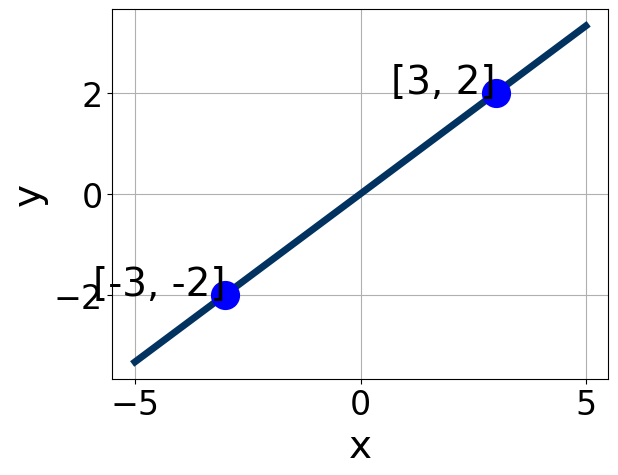
\includegraphics[width=0.5\textwidth]{../Figures/linearGraphToStandardCopyA.png}
\end{center}
\begin{enumerate}[label=\Alph*.]
\item \( A \in [1.8, 6.1], \hspace{3mm} B \in [5, 10], \text{ and } \hspace{3mm} C \in [-17, -7] \)
\item \( A \in [-1.9, 2.9], \hspace{3mm} B \in [1, 3], \text{ and } \hspace{3mm} C \in [-3, -1] \)
\item \( A \in [-1.9, 2.9], \hspace{3mm} B \in [-3, 0], \text{ and } \hspace{3mm} C \in [1, 6] \)
\item \( A \in [1.8, 6.1], \hspace{3mm} B \in [-9, -4], \text{ and } \hspace{3mm} C \in [10, 18] \)
\item \( A \in [-4.1, -2.3], \hspace{3mm} B \in [-9, -4], \text{ and } \hspace{3mm} C \in [10, 18] \)

\end{enumerate} }
\litem{
Solve the linear equation below. Then, choose the interval that contains the solution.\[ \frac{4x + 6}{3} - \frac{7x + 7}{2} = \frac{-7x -3}{8} \]\begin{enumerate}[label=\Alph*.]
\item \( x \in [-1.7, -0.1] \)
\item \( x \in [1, 2.1] \)
\item \( x \in [0.1, 0.6] \)
\item \( x \in [3.8, 5.3] \)
\item \( \text{There are no real solutions.} \)

\end{enumerate} }
\litem{
First, find the equation of the line containing the two points below. Then, write the equation in the form $ y=mx+b $ and choose the intervals that contain $m$ and $b$.\[ (-4, -9) \text{ and } (-6, 11) \]\begin{enumerate}[label=\Alph*.]
\item \( m \in [-11, -7] \hspace*{3mm} b \in [-59, -45] \)
\item \( m \in [-11, -7] \hspace*{3mm} b \in [-8, 2] \)
\item \( m \in [-11, -7] \hspace*{3mm} b \in [48, 58] \)
\item \( m \in [9, 16] \hspace*{3mm} b \in [69, 76] \)
\item \( m \in [-11, -7] \hspace*{3mm} b \in [15, 23] \)

\end{enumerate} }
\litem{
Write the equation of the line in the graph below in Standard Form $Ax+By=C$. Then, choose the intervals that contain $A, B, \text{ and } C$.
\begin{center}
    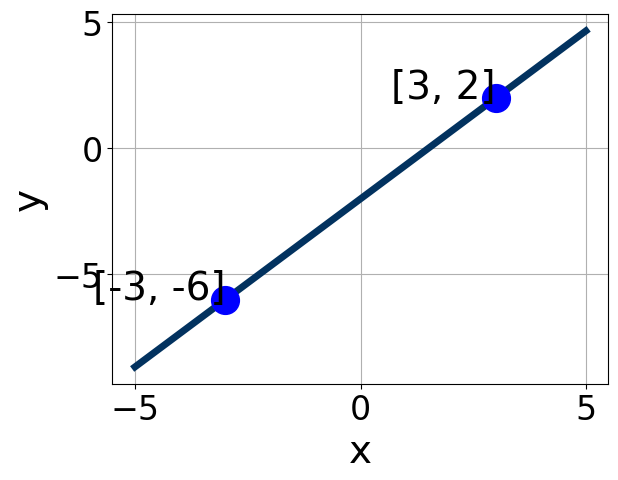
\includegraphics[width=0.5\textwidth]{../Figures/linearGraphToStandardA.png}
\end{center}
\begin{enumerate}[label=\Alph*.]
\item \( A \in [-2.8, 0.3], \hspace{3mm} B \in [-1.56, -0.72], \text{ and } \hspace{3mm} C \in [1.9, 5.3] \)
\item \( A \in [-2.8, 0.3], \hspace{3mm} B \in [-0.23, 1.48], \text{ and } \hspace{3mm} C \in [-4.6, -0.6] \)
\item \( A \in [-5.5, -1.4], \hspace{3mm} B \in [1.28, 4.39], \text{ and } \hspace{3mm} C \in [-7.8, -5.5] \)
\item \( A \in [1.5, 5.9], \hspace{3mm} B \in [-4.02, -2.82], \text{ and } \hspace{3mm} C \in [5.5, 8.2] \)
\item \( A \in [1.5, 5.9], \hspace{3mm} B \in [1.28, 4.39], \text{ and } \hspace{3mm} C \in [-7.8, -5.5] \)

\end{enumerate} }
\litem{
Solve the equation below. Then, choose the interval that contains the solution.\[ -18(3x + 7) = -17(10x + 13) \]\begin{enumerate}[label=\Alph*.]
\item \( x \in [-3.46, -2.92] \)
\item \( x \in [-1.84, -0.97] \)
\item \( x \in [-1.35, -0.48] \)
\item \( x \in [2.86, 3.64] \)
\item \( \text{There are no real solutions.} \)

\end{enumerate} }
\litem{
First, find the equation of the line containing the two points below. Then, write the equation in the form $ y=mx+b $ and choose the intervals that contain $m$ and $b$.\[ (-3, -4) \text{ and } (4, 6) \]\begin{enumerate}[label=\Alph*.]
\item \( m \in [1.1, 4.2] \hspace*{3mm} b \in [-1.52, -0.75] \)
\item \( m \in [1.1, 4.2] \hspace*{3mm} b \in [-0.47, -0.2] \)
\item \( m \in [1.1, 4.2] \hspace*{3mm} b \in [1.45, 2.09] \)
\item \( m \in [-4.7, 1.2] \hspace*{3mm} b \in [11.62, 11.75] \)
\item \( m \in [1.1, 4.2] \hspace*{3mm} b \in [0, 0.79] \)

\end{enumerate} }
\litem{
Solve the linear equation below. Then, choose the interval that contains the solution.\[ \frac{-3x + 5}{3} - \frac{8x + 8}{7} = \frac{-5x + 7}{4} \]\begin{enumerate}[label=\Alph*.]
\item \( x \in [-0.5, 0.1] \)
\item \( x \in [-11.5, -10.9] \)
\item \( x \in [0.9, 1.9] \)
\item \( x \in [-3.1, -1] \)
\item \( \text{There are no real solutions.} \)

\end{enumerate} }
\end{enumerate}

\end{document}